\documentclass[a4paper, final, 12pt]{article}
%%%%%%%%%%%%%%%%%%%%%%%%%%%%%%%%%%%%%%%%%%%%%%%%%%%%%%%%%%%%%%%%%%%%%%%%%%%%%%%%%%%%%%%%%%%%%%%%%%%%%%%%%%%%%%%%%%%%%%%%%%%%%%%%%%%%%%%%%%%%%%%%%%%%%%%%%%%%%%%%%%%%%%%%%%%%%%%%%%%%%%%%%%%%%%%%%%%%%%%%%%%%%%%%%%%%%%%%%%%%%%%%%%%%%%%%%%%%%%%%%%%%%%%%%%%%
\usepackage{eurosym}
\usepackage{amsmath, amssymb, latexsym, amscd, amsthm,amsfonts,amstext}
\usepackage[mathscr]{eucal}
\usepackage{graphicx}
\usepackage{subfig}
\usepackage{float}
\usepackage{color}
\usepackage{hyperref}
\usepackage[utf8]{inputenc}
\usepackage[english]{babel}

\setcounter{MaxMatrixCols}{10}
%TCIDATA{Version=5.50.0.2960}
%TCIDATA{<META NAME="SaveForMode" CONTENT="1">}
%TCIDATA{BibliographyScheme=Manual}
%TCIDATA{LastRevised=Thursday, February 17, 2022 21:02:18}
%TCIDATA{<META NAME="GraphicsSave" CONTENT="32">}
%TCIDATA{Language=American English}
%TCIDATA{ComputeDefs=
%$u_{xx}=\left( v_{xx}+2\lambda v_{x}+\lambda ^{2}v\right) e^{\lambda \left(
%x+\alpha t\right) },u_{xt}=\left( v_{xt}+\lambda \alpha v_{x}+\lambdav%
%_{t}\right) $
%}


 \textwidth = 16cm
 \textheight = 24cm
 \topmargin = -1cm
 \headsep =20pt
 \oddsidemargin = 15pt
 \evensidemargin = -15pt
 \renewcommand{\baselinestretch}{1} 
\newtheorem{theorem}{Theorem}[section]
\newtheorem{lemma}{Lemma}[section]
\newtheorem{problem}{Problem}[section]
\newtheorem{definition}{Definition}[section]
\newtheorem{algorithm}{Algorithm}[section]
\newtheorem{corollary}{Corollary}[section]
\newtheorem{remark}{Remark}[section]
\numberwithin{equation}{section}
 \pagestyle{myheadings}
\newcommand{\R}{\mathbb{R}}
\newcommand{\C}{\mathbb{C}}
\newcommand{\ds}{\displaystyle}
\newcommand{\Div}{{\rm div}}
\newcommand{\Curl}{{\rm curl}}
\newcommand{\usc}{u_{\rm sc}}
\newcommand{\width}{5cm}
\newcommand{\height}{4.5cm}
\newcommand{\ii}{{\rm i}}
\newcommand{\ik}{\ii k}
\newcommand{\eps}{\varepsilon}
\newcommand{\x}{{\bf x}}
\newcommand{\y}{{\bf y}}
\renewcommand{\d}{\mathrm{d}}
\begin{document}
\title{HIV Modeling}
\author{Michael Lie, Elizabeth Bui, Kathleen Cahya, and Matthieu Durieux}
\maketitle
\begin{abstract}
This paper presents three different HIV models: the SI model, the SID model, and the SIC model. The SID model and SIC model build upon the SI through the addition of a death (D) and C (cure) function. For the SID and SIC models, a mixture of numerical analysis and mathematical methods are used to provide insight into the shape and form of the models. The results of all models show one of two results: everyone dies or HIV is eradicated. Comparing these results to tabular data from the CDC proved inconclusive as HIV the CDC data proved more linear in fashion. These results indicate the potential great efficacy of a cure in a theoretical environment as well as the inaccuracies of the model compared to real life. 

\end{abstract}
\section{Introduction}\label{sec:Introduction}
\hspace{22pt} Human immunodeficiency virus, or HIV for short, “is a virus that attacks the immune system”, that if left untreated, can lead to acquired immunodeficiency syndrome, or AIDS [1]. In the late 1800s, HIV is hypothesized to have jumped from chimpanzees to humans, starting its spread in Africa before making its way to the United States by the 1970s [1]. As of 2020, the CDC estimated 1,189,700 people had HIV in the United States [1], with 30,635 people being newly diagnosed [1]. \\

HIV is transmitted when HIV-contaminated blood, semen, pre-seminal fluid, rectal fluids, vaginal fluids, or breast milk [1] come into contact with mucous membranes or damaged tissues or are injected into one's bloodstream. HIV is not transmitted through bodily fluids like saliva, tears, sweat, or other mediums like air and insects [1]. One also cannot get HIV by consuming food handled by someone infected with HIV, getting a tattoo, having physical contact with someone infected with HIV [1], drinking from a public water fountain, or donating blood [9].\\

Once one is infected with HIV, one begins in the first of three stages of HIV infection: acute infection. In this stage, one has flu-like symptoms, which upon testing, will confirm HIV status [1]. During acute infection, one's viral load, the amount of HIV in the bloodstream, is the highest which makes this stage the most transmittable [1]. Should one fail to receive proper treatment, one's infection will upgrade into a chronic HIV infection, also known as asymptomatic infection or clinical latency [1]. At this stage, one can still spread HIV, but they no longer have flu-like symptoms from acute infection. Persons who receive treatment at this point are unlikely to progress to AIDS. However, should one not receive treatment, their HIV will become AIDS. AIDS is defined to occur when one's CD4 cells, a type of white blood cell, fall below 200 cells/mm3 of blood (compare to the normal 500 - 1600 CD4 cells/mm3 of blood) or when one develops an opportunistic infection [9]. At this point, persons with AIDS have extremely damaged immune systems, and are very susceptible to opportunistic infections [1] like Herpes Simplex virus 1 (HSV-1), Salmonella infection, Tuberculosis, etc. [4]. Without intervention, people infected with AIDS survive for around 3 years [1]. \\

At this point in time, there is no available cure; if HIV infects one, one will have it for life [1]. However, while one can never cure oneself of HIV, as mentioned above, multiple treatments are available to help mitigate HIV effects and prevent spread [1], as well as medicines that can prevent one from being infected. Treatments for HIV, like antiretroviral therapy (ART) [9], aim to reduce one's viral load to an undetectable viral load [1]. Viral suppression is defined as less than 200 copies of HIV/ ml blood [9]. Through treatment, most people are able to attain an undetectable viral load within 6 months of treatment [9], and after can live a full life with no risk of spreading HIV [1]. For persons at risk of, but not yet infected with, HIV, medicines are available to prevent HIV pre- and post-exposure. Pre-exposure, and pre-exposure prophylaxis (PrEP) [9] can be used to prevent HIV from taking hold within one's body risk from getting HIV [6]. PrEP, when taken regularly, can reduce the risk of HIV infection by about 99\% from sex and 74\% from drug injection [6]. Within the first 72 hours post-exposure, post-exposure prophylaxis (PEP) medicine can prevent HIV from taking hold [9]. Should PEP be taken after 72 hours, it will no longer be effective [5]. Unlike PrEP, PEP is only for emergencies and must be taken for 28 days with less than a 100\% guarantee of effectiveness [5].\\

Though HIV is unlikely to kill one directly, it makes one more susceptible to opportunistic infections [9] and other viruses and diseases like COVID-19 [2]. The best way to prevent this situation altogether is to quickly test and provide medicine ASAP for maximum effect [9]. \\

One way to ensure adequate testing and resources as available is through accurate HIV models. HIV models help visualize HIV spread, showing the scope of infection and the effectiveness of treatments. This visualization will allow governments and other powers to prepare enough testing and treatment resources to fight against HIV. For others, it will help show the true expanse of the issue, hopefully encouraging people to pay due attention. As models become more accurate, they will become more effective at doing the above. In addition, models can also be used to test the effectiveness of different interventions and identify the most effective approaches for controlling the spread of HIV and improving outcomes for people living with the virus. This project aims to both improve upon and test the potential effectiveness of treatment by improving on an SI HIV model and through the inclusion of a potential cure and vaccination and treatment variables. \\

This project will present three different models of HIV: the SI model, the SID model, and the SIC model. The first model, the SI model, will serve as a baseline comparison to test the increased accuracy of the following models. This model is derived from AMATH 383's section 1.3 on Logistic Growth. The SI model has the following guiding equation,
    \begin{align}
        S(t) + I(t) = N
    \end{align}
\hspace{22pt} Where N is some constant population, I(t) is the number of infected individuals, and S(t) is the number of susceptible individuals. This model makes a few key assumptions. One, it assumes that HIV is non-lethal. Two, everyone not infected is susceptible to infection. In other words, there is no cure or possible recovery. Three, the population is closed and constant; there are no births, deaths, nor migrations into the population. \\

These assumptions and equation result in the following logistic growth model:
\begin{align}
    \frac{dI}{dt} = r I (1 - \frac{I}{N})
\end{align}
    \begin{center}
        \(r > 0: \) \textit{the rate of infection.}
    \end{center}

The second model is the SID model, which builds upon the SI model with the term d(t), the number of people who died from HIV/AIDS. This model is inspired by Ayele's, et al.[8], inclusion of a death rate. The inclusion of death will help improve the real-life accuracy of the SI model. The SID model has the following guiding equation:
    \begin{align}
        S(t) + I(t) + D(t) = N
    \end{align}
\hspace{22pt} This model makes slightly different assumptions from the first model. First, HIV is lethal and will result in death. Second, everyone not infected is susceptible to infection. Third, the population is closed and constant. \\

These assumptions and equations result in the following model:
\begin{align}
    \frac{dS}{dt} = -\alpha SI \\
    \frac{dI}{dt} = \alpha SI - \gamma I \\
    \frac{dD}{dt} = \gamma I
\end{align}
\begin{center}
    \(\gamma > 0: \) \textit{the rate of mortality.}\\
    \(\alpha > 0: \) \textit{the rate of infection.}
\end{center}
\hspace{22pt}
The final model presented will be the SIC model, which builds upon the SI model with the term C(t), representing cured, immune, or recovering persons in a population. This model takes the idea of a removed population, r(t), from Arias et al [7] and extrapolates it to include the idea of a, currently, non-existent cure. While the study [7] assumed r(t) is negligible, as no one is permanently immune, this project chooses to circumvent this assumption by presuming a non-existent cure, as well as by including currently available preventative measures, that are, as mentioned above, up to 99\% effective in certain circumstances. It also takes from an Ethiopian study [8] the idea of an educated population. The inclusion of a cure in this model will help test the potential efficacy of a cure, as well as test other factors like education, preventative medicines, and HIV treatments.  These factors result in the guiding equation
    \begin{align}
        S(t) + I(t) + C(t) = N(t)
    \end{align}
 Where N(t), the population at time t is subdivided into three subclasses. \\
\textit{
S: the susceptible population increases due to natural birth and lack of education and decreases due to infection and vaccination. \\
I: the infected population, which can increase due to infection, and decreases due to recovery and death. \\
C: the cured, immune, and treated population. \\
}

There are four key assumptions this model makes. First, HIV is lethal and will result in death. Second, someone who is cured can be reinfected. Third, the population can increase due to natural birth. Four, someone who takes an HIV-prevention medicine, PrEP, cannot get HIV, and is effectively vaccinated against infection. \\
Taking these assumptions into account results in the following model: 
\begin{align}
    \frac{dS}{dt} = -\beta SI - \mu S + \eta + \epsilon C \\
    \frac{dI}{dt} = \beta SI - \delta I \\
    \frac{dC}{dt} = \gamma I + \mu S + \eta - \epsilon C
\end{align}
\begin{center}
    \(\delta = \gamma + d \) \\
    \(\beta > 0: \) \textit{rate of infection.}, \(\mu > 0: \) \textit{rate of vaccination.} \\
    \(\eta > 0: \) \textit{constant birth rate.}, \(\gamma > 0: \) \textit{rate of recovery.} \\
    \(\epsilon > 0: \) \textit{rate of uneducation.}, \(\d > 0: \) \textit{death rate.}\\
\end{center}

\subsection{Thesis Statement}
\hspace{22pt} This paper aims to improve the real-life accuracy of the SI model through the additions of death and cure as a function of time. Further analysis will be done to estimate the dynamics of the models with changing variables. In the first section, the data and equations used to complete the analysis will be outlined. The following section will implement the prior section's methods and data to analyze HIV infection under different circumstances. The last sections discusses the benefits, limitations, and future research pathways of this project. 

\section{Data and Methods}
\hspace{22pt} The SI model will provide the foundation to the following models. With the graph of this model, one cane see how the population of the susceptible perform with the population of the infected. In addition, this graph will be compared with a graph of the number of infected people per year between 2015-2019 created from the CDC's Estimated HIV Incidence and Prevalence report [3].\\

The second mode consists of equations 1.4, 1.5, and 1.6. As the equation makes the assumptions $I(0)=I_0 > 0$, $S(0)=S_0 > 0$, $r(0)=0$, one can solve for the infection function over time I(t) in terms of the susceptible function S(t). \\
$$\frac{dI/dt}{dS/dt} = \frac{\alpha SI-\gamma I}{-\alpha S I}$$\\
$$\frac{dI}{dS} = -1 + \frac{\gamma}{\alpha S}$$\\
$$dI = (\frac{\gamma}{\alpha S} - 1)dS$$\\
$$\int dI = \int (\frac{\gamma}{\alpha S} - 1)dS$$\\
$$I = \frac{\gamma }{\alpha}ln|S|-S+K$$\\
Let $\frac{\gamma}{\alpha} = \beta$, where \(\beta\) is the relative death rate. Thus,\\
$$I(t) = \beta ln|S(t)|-S(t)+K$$\\
Combining the assumed initial conditions together results in the following: \\
$$I(t) = P - S(t) + \beta ln|\frac{S(t)}{S_0}|$$
This will be the final equation for the Infection rate over time. 
Similarly, one could also solve for the susceptible function over time S(t) in terms of r(t). \\
$$\frac{dS/dt}{dr/dt} = \frac{-\alpha SI}{\gamma I}$$\\
$$\frac{dS}{dr} = -\frac{\alpha}{\gamma}S$$\\
$$\int \frac{1}{S}ds = \int -\frac{\alpha}{\gamma}dr$$\\
$$ln|S| = -\frac{\alpha}{\gamma}r+K$$\\
Let $\frac{\gamma}{\alpha} = \beta$, \\
$$S(t) = S_0e^{-\beta^{-1}r(t)}$$
This will be the final equation for the Susceptible rate over time. One can also find the maximum number of infected by taking the derivative of I(t). \\
$$\frac{dI}{dt} = 0$$\\
$$I' = -1 + \frac{\beta}{S(t)} = 0$$
$$S(t) = \beta $$
$$I_{max} = P - \beta + \beta ln|\frac{\beta}{S_0}|$$
$$S = S(R)$$
$$I = I(S)$$
$$\frac{d}{dt}I(S(t)) = 0$$
$$I'(S(t)) = 0$$\\

Furthermore, I(t), the Infection function over time, will be graphed and compared with the tabular data graph [3]. The result will allow be used to measure the performance of the model. \\

As for the third model, it will incorporate linear stability analysis using a 3x3 nonlinear systems. The linear stability analysis allows one to study the trajectories corresponding to different initial conditions, obtain information about the stability of the equilibrium, and measure solution performance in the long term. \\

To start with the linear stability analysis, one will first find the fixed points of the equations. \\\\
Setting the differential equation to 0 results in: \\
\begin{align}
    -\beta SI - \mu S + \eta + \epsilon C = 0 \\
    \beta SI - \delta I = 0 \\
     \gamma I + \mu S + \eta - \epsilon C = 0
\end{align}
By doing some algebra on (2.5), one can find s, \\
$$\beta S I - \delta I = 0$$\\
$$S = \frac{\delta}{\beta}$$
Substituting s back to (2.4) and (2.5) results in the following: \\
$$-\beta S I - \mu S + \eta + \epsilon C = 0$$\\
$$-\beta \frac{\delta}{\beta}I - \frac{\mu \delta}{\beta} + \eta + \epsilon C = 0$$\\
$$-\delta I - \frac{\mu \delta}{\beta} + \eta + \epsilon C = 0$$\\
$$-\delta I + \epsilon C = \frac{\mu \delta}{\beta} - \eta$$\\
$$\gamma I + \mu S - \epsilon C = 0$$\\
$$\gamma I + \frac{\mu \delta}{\beta} -\epsilon C = 0$$ \\
$$\gamma I - \epsilon C = -\frac{\mu \delta}{\beta}$$
With elimination of the two equations, one can get I, which will be substituted back into (2.6) to get C. Therefore, the fixed point is\\
\begin{equation} \label{eq1}
\begin{split}
    S^* & = \frac{\delta}{\beta} = \frac{\gamma + d}{\beta}\\
    I^* & = \frac{\eta}{\delta - \gamma} = \frac{\eta}{d}\\
    C^* & = \frac{\gamma \eta}{\epsilon d} + \frac{\mu (\gamma + d)}{\epsilon \beta}\\
\end{split}
\end{equation}
Where $\delta = \gamma + d$. Let\\
\begin{align}
    f(S,I,C) &= -\beta SI - \mu S + \eta + \epsilon C \\
    g(S,I,C) &= \beta SI - \delta I\\
     h(S,I,C) &= \gamma I + \mu S + \eta - \epsilon C
\end{align}
Using this information, one can find the Jacobian matrix, \\
$$ J = \begin{pmatrix} df/dS & df/dI & df/dC \\ dg/dS & dg/dI & dg/dC \\ dh/dS & dh/dI & dh/dC\end{pmatrix}$$
$$ J = \begin{pmatrix}-\beta I - \mu & -\beta S & \epsilon \\ \beta I & \beta S - \delta & 0\\ \mu & \gamma & -\epsilon \end{pmatrix}$$
Evaluating the Jacobian matrix at the fixed points results in\\
$$ J = \begin{pmatrix}-\frac{\beta \eta}{d} - \mu & -(\gamma + d) & \epsilon \\ \frac{\beta \eta}{d} & 0 & 0\\ \mu & \gamma & -\epsilon \end{pmatrix}$$
Now, one can then find the determinant of the matrix to find the eigenvalues, which will lead to the following characteristic polynomial:\\
$$\lambda^3+(\frac{\beta \eta}{d} + \mu + \epsilon)\lambda^2 + (\beta \eta(\frac{\epsilon + \gamma}{d}+1))\lambda + \beta \eta \epsilon = 0$$
Now, let\\
\begin{equation} \label{eq1}
\begin{split}
    a_2 & = \frac{\beta \eta}{d} + \mu + \epsilon\\
    a_1 & = \beta \eta (\frac{\epsilon + \gamma}{d}+1)\\
    a_0 & = \beta \eta \epsilon\\
\end{split}
\end{equation}
$$\lambda^3+a_2\lambda^2+a_1\lambda + a_0 = 0$$
\hspace{22pt}Suppose there exist $\lambda_* > 0$ such that $f(\lambda_*)=0$, then this is a contradiction. Therefore, there exists no possible positive real solutions. Then, this leads to two options: (i) three negative real solutions OR (ii) two complex conjugates with positive real parts and one negative solutions. The following section will examine the second option. \\
$$\lambda^3+a_2\lambda^2+a_1\lambda+a_0 = (\lambda-\lambda_1)[\lambda-(A+iB)][\lambda-(A-iB)]$$
\begin{equation} \label{eq1}
\begin{split}
    a_2 & = -\lambda_1-2A\\
    a_1 & = A^2+B^2+2A\lambda_1\\
    a_0 & = -\lambda_1(A^2+B^2)\\
\end{split}
\end{equation}
Solving the equations results in two different inequalities: $a_1 < B^2$ and $a_2B^2-a_0 < 0$. Combining these two inequalities together one can get $a_1<B^2<\frac{a_0}{a_2}$ resulting to $a_1a_2 < a_0$. \\
$$(\frac{\epsilon + \gamma}{d}+1)(\frac{\beta \eta}{d} + \mu + \epsilon) < \epsilon$$\\
$$\frac{\beta \eta (\epsilon + \gamma)}{d^2}+\frac{\mu(\epsilon+\gamma)}{d}+\frac{\epsilon(\epsilon + \gamma)}{d} + \frac{\beta \eta}{d}+\mu > 0$$\\
$$\beta \eta(\frac{\epsilon + \gamma}{d}+1) < -\mu(\epsilon + \gamma) - \epsilon(\epsilon + \gamma) - \mu d$$\\
$$\beta < \frac{-\mu(\epsilon + \gamma) - \epsilon(\epsilon + \gamma) - \mu d}{\eta ( \frac{\epsilon + \gamma}{d}+1)}$$\\
\hspace{22pt}Here, there is a contradiction as $\beta$ is some negative value, but this equation assumes that $\beta$, the rate of infection, is $\beta > 0$. Therefore, one can conclude that the option (ii) is invalid, which means that the eigenvalues should be negative real valued, resulting in a stable fixed point.\\


\section{Results}

\hspace{22pt} The variations of SI models such as the SID model (1.3) and the SIC model (1.7) build upon the standard SI model (1.1) and are intended to simulate HIV/AIDS disease situations as close to reality, under such circumstances, as possible. \\

\begin{figure}[!ht] 
    \centering
    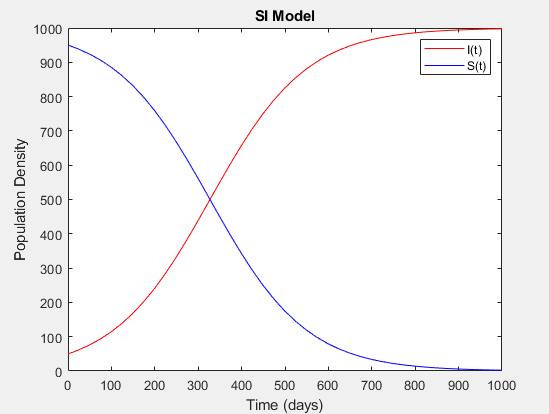
\includegraphics[width=0.6\textwidth]{image (2).png}
    \caption{Figure 1: SI Model Over 1000 days}
    \label{fig:matrix3}
\end{figure}

Figure 1 is the SI model (1.1) based on functions of the susceptible and infected people over time within a closed population. As time goes on ($t \to \infty$), the susceptible population will decrease at an exponential rate while the number of infected people will increase at an exponential rate making the whole population will move from the susceptible class to the infected class. This result shows that the population will end up being infected, meaning that there will be a pandemic of HIV/AIDS on a global scale. It is proven from the graph that all of the susceptible will transfer into the infected class and not allow the infected to go back to being susceptible. Therefore, this is the reason why the SI model is incomplete and non-realistic. One can increase realism by adding more dynamics to the SI model through various constants and variables such as the death $D(t)$ and $C(t)$ that will be discussed more below. With more constants and equations that replicate the complexity of real life, one can get closer to modeling HIV with higher accuracy. \\

\begin{figure}[!ht] 
    \centering
    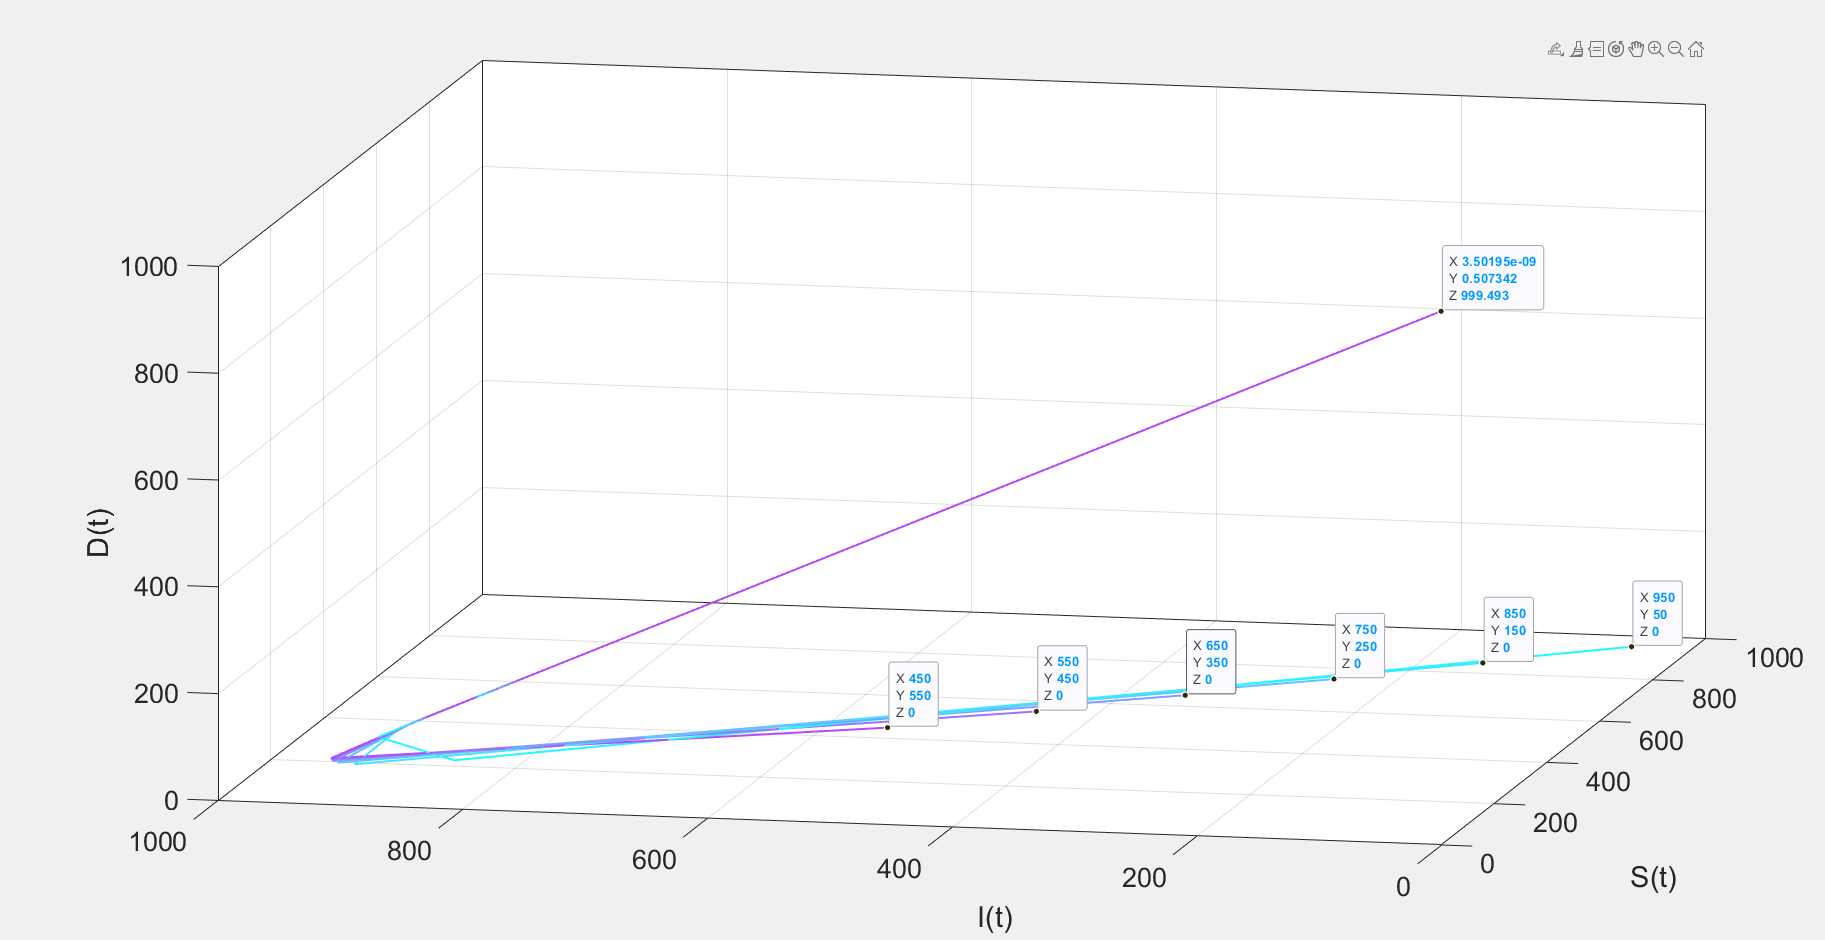
\includegraphics[width=0.7\textwidth]{model1.png}
    \caption{Figure 2: SID Model Over 1000 days}
    \label{fig:matrix3}
\end{figure}

The first build-up to the standardized SI model (1.1) is the SID model (1.3), in which the death variable $D(t)$ and mortality rate $\gamma$ are added to the SI model as explained in the introduction section. Recall that $I(0) > 0, S(0) > 0, D(0) = 0, \alpha > 0, \gamma > 0$; setting the infection rate to be $\alpha = 0.1$ and mortality rate $\gamma = 0.2$, figure 2 is showing that the whole population will move to the infected population and eventually the whole infected population will move to the death population. Varying the parameters and the initial conditions as shown in Figure 2 below would make no significant changes to how each fixed point will move as ($t->\infty$) which the population will entirely die due to the assumption that infected people can’t move back being susceptible, which they could only either stay infected and eventually die. \\

\begin{figure}[!ht] 
    \centering
    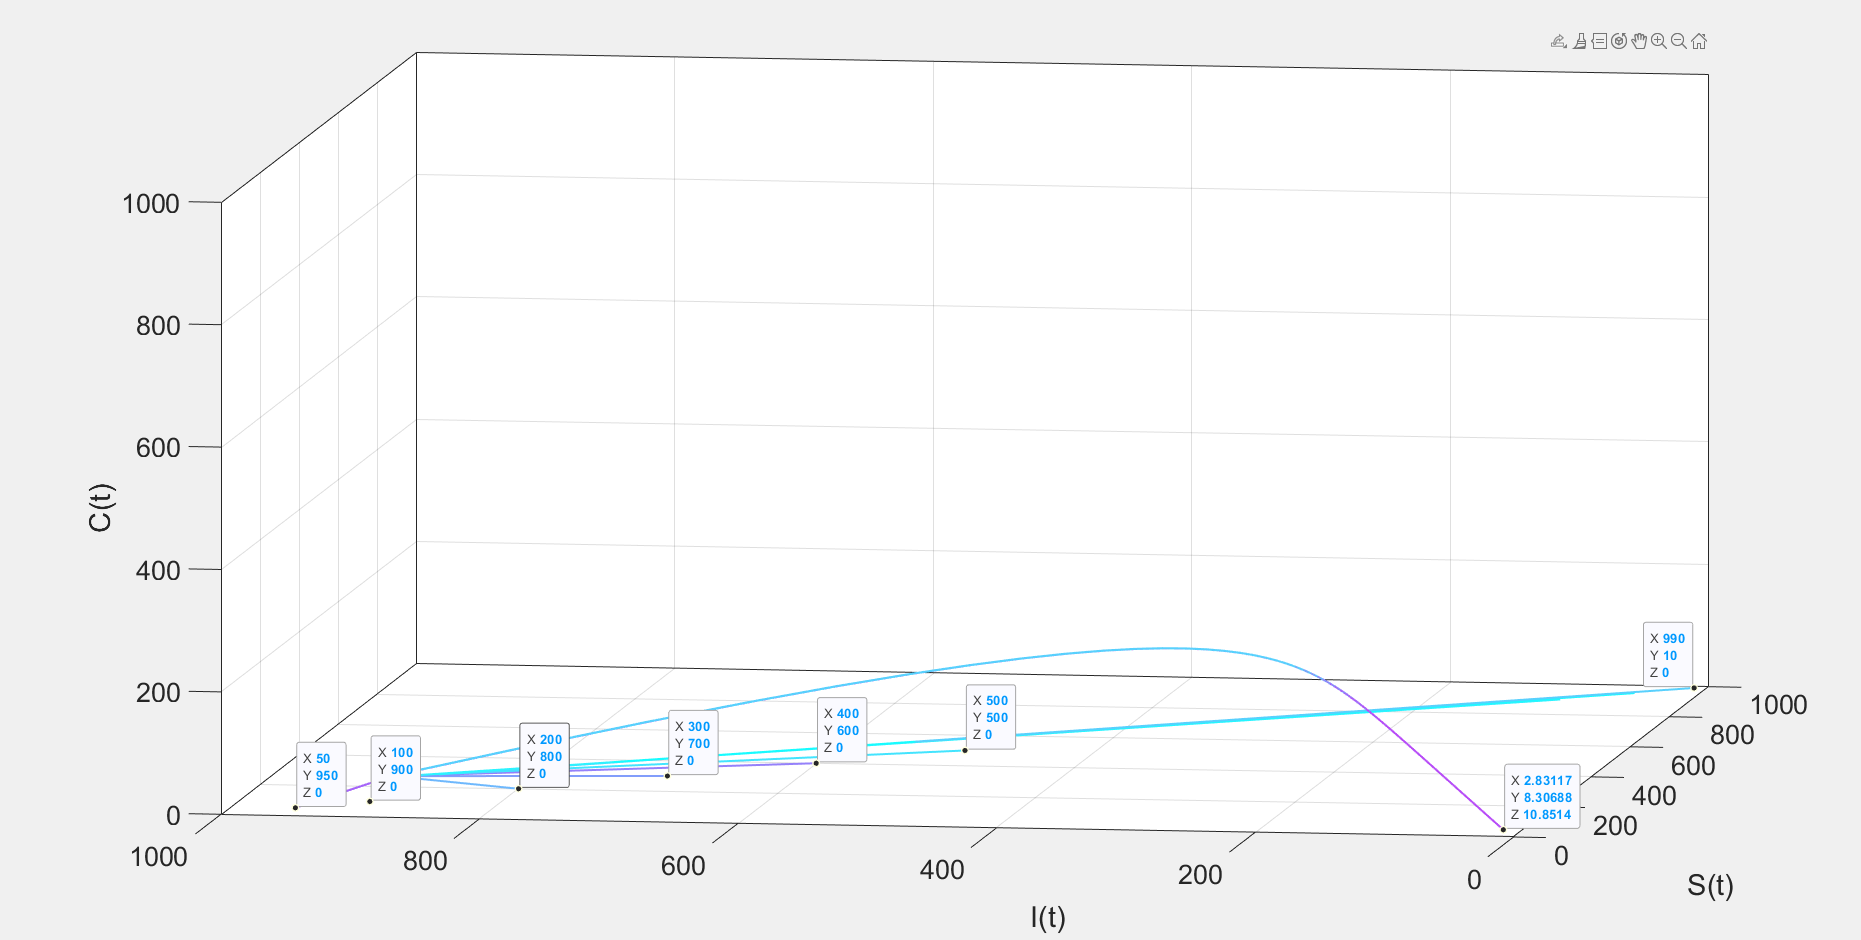
\includegraphics[width=0.7\textwidth]{model2.png}
    \caption{Figure 3: SIC Model Over 1000 days}
    \label{fig:matrix3}
\end{figure}

The third equation, a build-up from the standardized SI model as well as the SID model, is the SIC model, where the cured variable $C(t)$, rate of vaccination $\mu(t)$, constant birth rate $\eta$, recovery rate $\gamma$, rate of uneducated people $\eps$, and death rate $d$ are added to simulate the more realistic environment and dynamics of real-life situations. Figure 3 below exhibits the behavior of a SIC HIV/AIDS model that in the long term, the population will distribute among the susceptible, infected, and cured subclasses. Recall the assumptions made that the SIC model is an open population that allow a constant birth rate to enter the population while assuming there is a vaccine and cure for people that are transmitting HIV or even before contracting HIV/AIDS as well as allowing uneducated people from the cured population to go back being susceptible and in risk of contracting HIV again. Keeping the infected rate, vaccination rate, recovery rate, and uneducated rate constant ${0 \leq \beta, \mu, \eta, \gamma, \eps, d \leq 1: \beta = 0.1, \mu = 0.02, \eta = 1, \gamma = 0.05, \eps = 0.13}$ while varying the death rate [d], it can be seen that in the long run, the higher the death rate is, the more people stay within the infected population. This implies that more people are transmitting the HIV/AIDS while leaving from the susceptible yet, the cured population is less than the infected population. This is true if only if the rate of death $d$ is higher than the rate of recovery $\gamma$. Moreover, if gamma is relatively small and d is relatively large ($\gamma < d$) then the eigenvalues will be complex conjugate pairs with negative real parts as well as a negative real root indicating that the fixed points are a stable spiral whereas if $\gamma$ is relatively large and $d$ is relatively small ($\gamma > \d$) then the eigenvalues will always be real and negative, which indicates the fixed points are a stable node. \\

\begin{figure}[!ht] 
    \centering
    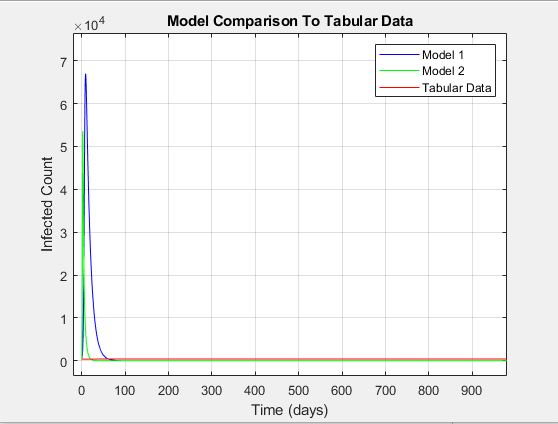
\includegraphics[width=.7\textwidth]{image (3).png}
    \caption{Figure 4: SID/SIC Models vs. Tabular Data}
    \label{fig:matrix3}
\end{figure}

Lastly, to draw the significance between both build-up SID and SIC models on the SI model, both models will be compared with the tabular data to measure the performance of the SID and SIC models against the real-world. Keeping the constant rates $\alpha = 0.00001$ and $\gamma = 0.1$ for the SID model while $\beta = 0.00004$ , $\mu = 0.02$ , $\eps = 0.6$ , $\gamma = 0.23$ , $d = 0.4$ , and $\eta = 0.9$ for SIC model, the model results exhibit a poor comparison with the tabular data. The tabular data is a linear model with approximately 36680 people each year, in which, if made proportional to a population with one thousand people, the linear equation for the tabular data will be $y = 0.0001105x + 4$. Considering that the equations are in the form of logistic growth, then the results gained from the models will be a poor comparison with the tabular data. \\

Furthermore, based on the constant difference, both of the models, the SID and SIC model, exhibit that due to our assumptions where if a cure and vaccination to HIV/AIDS is present then HIV would be eradicated or the model is proposing an endemic whereas if there is no cure or vaccination yet then the whole population would be eradicated or there will be a pandemic of HIV/AIDS, infecting the whole population, which the whole population will eventually dies out. One can see qualitatively that both of our models goes to zero for infected population $I(t)$ in an exponential rate, either the whole population are cured or dies out while the tabular data starts at 400 and increases by 0.1 every day. \\

\section{Discussion}\label{sec:theory}
\hspace{22pt} The first model, which is the original SI model, implies physically that over time the population will become infected. The limitation of this model is that this model does not consider the fact that there might be a cure in the near future, and the possibility of some of the population dying. Therefore, this model might not be as accurate as the other two models. With the extended SI model, which are the SID and SIC models, one can further investigate how the multiple parameters like death and cure rate comes into play. These multiple parameters allow one to make the results from the extended model closer to the actual data; thus, increasing the model’s accuracy. The SID model considers the possibility of death, and based on the model, the HIV/AIDS will lead everyone in the population to die in the long term. This model is significant because one can use the model to measure death due to HIV/AIDS, in which the model predicts that everyone in the closed population to die. However, to make this more realistic, one can use the SIC model. The SIC model both incorporates the death rate as well as the cured rate. Other than that, there are also have a few parameters that come into play, such as the rate of uneducated people, birth rate and the rate of vaccination. This model is significant because in the near future, there might be a vaccination for HIV/AIDS in which people can be cured from the disease. However, with the added parameter of the rate of uneducated people, some of the population that are already cured can become susceptible again. The SIC model is most realistic out of the three since it incorporates different factors in the model which can improve the model’s accuracy. Since there is no cure or vaccine yet for the HIV model, one cannot really compare our SIC model to the tabular data. However, logically, the results are correct because if there is a cure to the HIV model, then the population will be cured over time. \\

The SI model accounts for the infected and susceptible people, which means that the population will be infected as time goes to infinity. The SID model agree with the fact that the population will become infected with HIV/AIDS over time, but it disagrees with the SI model since in the model, people will eventually die if they get infected in the long run with the assumption that there is no cure and vaccine. As for the SIC model, it also agrees with the fact that the population will become infected over time, but it disagrees with the assumption that now the model is an open population and now that there is a cure or vaccine, some people will be cured.\\

To analyze the third model, linear stability analysis was used to evaluate the stability of the fixed point. However, one of the limitations to this method is that it is hard to find the eigenvalues and predict the stability of the fixed point since this is a 3x3 systems. Assumptions needed to be made that may lead to a contradiction. Furthermore, there is an inefficiency in the method of trial and error for the constant values so that the result is similar to that of the tabular data. Although the added parameters in the third model can make our model accurate as in closer to our tabular data, it takes a lot of time and effort to determine the correct values for the parameters. If given enough time, the model could be improved by using a multiple linear regression in order to estimate the parameters so that the error between the model and the actual data is minimal. In this case, the model would be even more accurate to the actual data.\\

\section{Conclusions}\label{sec:Gini}
\hspace{22pt} In this paper, there were two model iterations considered that were build upon the standardized SI model, the SID model that incorporates death variable $D(t)$ to simulate situations of when HIV/AIDS disease circulating within the population and the SIC model that incorporates cured variable $C(t)$ to simulate situations based on our early assumptions made to the model where this is no longer a closed population, which allows for a constant birth rate to enter the population (opened population), vaccinations and cure to allow susceptible and infected people to enter the cured population, uneducated people that lacks of HIV/AIDS knowledge or unaware of the different scenarios that they might encounter that would make them contract and transmit the HIV/AIDS as well as mortality rate of people dying from the disease over time. By comparison, the first observation key from the SI model is that over time, the whole population will go from susceptible into being infected of HIV/AIDS. The second key observation on the SID model exhibit that in the long run, every one in the population will goes from being infected into dying out resulting a pandemic. The third key observation on the SIC model shows that when $t -> \infty$ there are different scenarios that could happen due to varying the constant rates such as: when $d > \gamma$ then when $t -> \infty$ the population will mostly stays in I(t) or being infected, and in contrary, when $d < \gamma$ then when $t -> \infty$ then the population will recover from the disease. Both situations draw simulations of a pandemic will happen if $d > \gamma$ whereas an endemic will happen when $d < \gamma$. The fourth key observation of the fixed points' stabilities exhibit that if the recovery rate is relatively smaller than the rate of death, the eigenvalues resulted in a complex conjugate pairs with negative real parts and a negative real part (cubic equation), meaning that the fixed points are stable spirals. On the other hand, when the rate of death is relatively smaller than the recovery rate, then the eigenvalues resulted in three negative real parts exhibiting that the fixed points have stable node stabilities. Both situations are implying similar situations where the fixed points will be stable over time, meaning that at the fixed point $(S_{*}, I{*}, C_{*}) = (\frac{\delta}{\beta} = \frac{\gamma + d}{\beta}, \frac{\eta}{\delta - \gamma} = \frac{\eta}{d}, \frac{\gamma \eta}{\epsilon d} + \frac{\mu (\gamma + d)}{\epsilon \beta})$ have a stable behavior over time. \\

Furthermore, the fifth key observation after comparing both SID and SIC models to the tabular data in real time, it shows that $I(t)$ within the models decreases at an exponential rate over time and having $I(t) = 0$ when $t -> \infty$ because of the assumptions that the population can die and the death population would still be included in the total population (SID model) while the population can be cured, assuming that there is a cure and vaccination for the disease (SIC model). However, the tabular data exhibits that the $I(t)$ would never reaches zero as time goes on because there is still no cure and vaccines that have been proven tested and released for the HIV/AIDS disease. The observation above implies that our models are not fully accurate to the real world situation of HIV/AIDS, because the prevalence and infection of HIV are impacted by many different factors such as location, sex, religion, poverty, drug usage in the area, current preventative measures, and ignorance of HIV. \\

However, the model iterations of SID and SIC model above the SI model exhibits the improvement of the real-life accuracy of the SI model through the variable additions of death and cure as functions of t because through adding the variables, one is able to simulate different scenarios and situations of the HIV/AIDS as well as adding more dynamics to what might happen rather than just concluding that the whole population will be infected as time goes on based on the standardized SI model. In addition, several improvements are noted for future research regarding the SI disease model for HIV/AIDS by using multiple regression analysis in order to estimate the parameters so that the error between the model and actual data is minimal, and adding more variables along with more accurate constants to coherently and rigorously produce better estimates according to various simulations of the HIV/AIDS disease modeling. \\




\pagebreak
\section{Bibliography}

\begin{thebibliography}{99}

\bibitem{CDC HIV Basics}
\textit{HIV Basics}, CDC (last reviewed 2022), \url{https://www.cdc.gov/hiv/basics}.
 
\bibitem{WHO infographic}
Infographic, World Health Organization (n.d.), \url{https://www.who.int/images/default-source/campaigns/aids-day-2021/who-social-03_1080.png?sfvrsn=5dc2ac74_5}.

\bibitem{HIV tabular}
\textsc{L. Laurie et al.} \emph{"Estimated HIV incidence and prevalence in the United States, 2015–2019"}, Division of HIV/AIDS Prevention, National Center for HIV/AIDS, Viral Hepatitis, STD, and TB Prevention, Centers for Disease Control and Prevention (CDC), U.S. Department of Health and Human Services, Atlanta, Georgia (2021).

\bibitem{Op Infections}
\textit{Opportunistic Infections}, HIV.gov (2022), \url{https://www.hiv.gov/hiv-basics/staying-in-hiv-care/other-related-health-issues/opportunistic-infections}.

\bibitem{PEP}
\textit{Post-Exposure Prophylaxis}, HIV.gov (2022), \url{https://www.hiv.gov/hiv-basics/hiv-prevention/using-hiv-medication-to-reduce-risk/post-exposure-prophylaxis }.

\bibitem{PrEP}
\textit{Pre-Exposure Prophylaxis}, HIV.gov (2021), \url{https://www.hiv.gov/hiv-basics/hiv-prevention/using-hiv-medication-to-reduce-risk/post-exposure-prophylaxis}.

\bibitem{Basic HIV model}
\textsc{R. Arias et al.} \emph{“Mathematical Modeling of the HIV-AIDS Epidemic”}, Open Access Library Journal (2022).

\bibitem{Ethiopia Model}
\textsc{T. Ayele et al.} \emph{“Mathematical modeling of HIV/AIDS with optimal control: A case study in Ethiopia”}, Elsevier B.V. (2021).

\bibitem{HIV Basics, HIV.gov}
\textit{What are HIV and AIDS?}, HIV.gov (2022), \url{https://www.hiv.gov/hiv-basics/overview/about-hiv-and-aids/what-are-hiv-and-aids}.

\end{thebibliography}
\end{document}